
\documentclass[a4paper,12p]{paper} 
\usepackage[margin=2.5cm]{geometry}
\usepackage{amsmath}
\usepackage{graphicx}
\usepackage{algorithm}
\usepackage{lipsum}
\usepackage{xcolor}
\usepackage{booktabs}
\usepackage{float}
\usepackage{subfigure}
\usepackage{titling}
\usepackage{kotex}
\usepackage{threeparttable}
\usepackage[newfloat]{minted}
\usepackage{caption}
\usepackage{tikz}
\usetikzlibrary{graphs, graphdrawing, automata,positioning}
\usegdlibrary{layered, force}
\usepackage{forest}

\newenvironment{code}{\captionsetup{type=listing}}{}
\SetupFloatingEnvironment{listing}{name=Listing}

\def\code#1{\texttt{#1}}
\sectionfont{\large\sf\bfseries\color{black!70!blue}}
\date{\vspace{-5ex}}
\renewcommand{\familydefault}{\sfdefault}
\renewcommand{\baselinestretch}{1.3} 

\pretitle{\centering\LARGE\bfseries}
\posttitle{\par}
\preauthor{\begin{flushright}\large}
\postauthor{\end{flushright}}

\title{컴파일러 프로젝트 4 결과보고서}
\author{컴퓨터공학과 20171634 박건\\전자공학과 20161453 김규래}

\begin{document} 
\maketitle\hrule{}\bigskip

\begin{center}
\begin{tabular}{ l l }
과목코드 & CSE4120 \\
과목명  & 기초 컴파일러 구성 \\
담당교수 & 정성원 \\
\end{tabular}
\end{center}

\section{개발 목표}
C Language를 간소화한 언어인 C- Language를 MIPS R2000 프로세서의 어셈블리로 컴파일한 다음, SPIM 을 통해 실행해보는 것이다. 이번 과제를 끝으로 MIPS 타겟의 컴파일러가 완성된다.

\vspace{0.1in}
\noindent\textbf{Runtime Environment:} 프로그램을 프로세서에서 실행하기 위해서는 보통 실행에 필요한 메모리나 정보들을 관리하여야 하는데, 이것들을 \textit{runtime environment} (RE) 라고 부른다. 이번 프로젝트에서 컴파일을 하는 C- 언어는 \textit{Procedural} (구조지향, 절차지향) 언어로, runtime stack, subroutine, array, variable scope 와 같은 기능들을 제공한다. 이러한 하이레벨 기능들은 모두 RE 에서 관리를 해줘야 사용이 가능하며 관련된 코드를 생성하는 것은 컴파일러의 몫이다. 또한, procedural 언어들은 매우 광범위하게 사용되기 때문에 하드웨어에서 관련 기능들을 제공해주는 경우가 많은데, MIPS 에서는 \textit{stack-pointer} (sp), \textit{frame-pointer} (fp) 등을 제공해준다.

\vspace{0.1in}
\noindent\textbf{Activation Record:} C- 언어에서 RE 를 관리하기 위해서 사용하는 자료구조를 \textit{activation record} (AR) 이라고 한다. AR 은 각 스코프별로 하나씩 생성이 되며, 함수호출시에 전달하는 parameter들, 함수 호출시에 반환 주소, 각 스코프의 지역변수들, 그리고 callee 의 AR 주소인 control link 를 담는다. Nested procedure call 을 사용하는 경우에는 \textit{access link} 를 사용하는데, C- 에서는 지원을 하지 않기 때문에 사용하지 않는다.

\vspace{0.1in}
\noindent\textbf{Code Generation:} 보통의 컴파일러들은 어떤 하이레벨 언어로 작성된 프로그램을 하드웨어가 쉽게 실행할 수 있는 로우레벨 언어로 변환을 해주는 역할을 하는데, 하이레벨 프로그램을 분석하고 (scanning, parsing, semantic alanyzing) 을 모두 마친 뒤에 \textit{Abstract Syntax-Tree} AST 로부터 어셈블리를 생성해주는 과정을 \textit{code generation} (CG) 이라고 부른다. \textit{Intermediate representation} (IR) 등을 거쳐서 CG 를 하는 경우가 많으나, 이번에는 C- 언어로부터 얻어낸 AST 로부터 바로 MIPS 어셈블리로의 CG 를 수행한다. IR 의 경우에는 실제 assembly 에 비해서 abstract 하기 때문에, 어셈블리를 사용할 때는 calling convention 이나 register allocation 같은 작업을 추가로 수행해야 하드웨어에서 컴파일한 프로그램을 정상적으로 실행할 수 있다.

\vspace{0.1in}
\noindent\textbf{Calling Convention:} Procedural 언어들의 핵심 기능중에 하나는 subroutine call, function call 또는 procedure call 이다. Procedure call 을 수행하기 위해서는 runtime environment 상으로 몇가지의 추가적인 작업들을 수행하여야 하는데, 이를 calling convention 이라고 부른다. 본 과제에서 사용한 calling convention 은 이후에 다룬다.


\section{개요}
본 프로젝트에서는 수업 교재 \textit{Compiler Construction Principles and Practices} 에서 제공하는 파일들을 포함하여 다음과 같은 프로젝트 파일 구성을 갖고 있다. 프로젝트 디렉토리 구성은 Tab.~\ref{table:files} 에 정리돼 있다. 본 프로젝트에서 작성한 파일들은 * 로 표시하였다. 

\begin{table}[H]
  \centering
\begin{threeparttable}
  \caption{프로젝트 파일 구성}\label{table:files}
\begin{tabular}{ll}
  \toprule
파일명 &    내용 \\
        \midrule
  \textbf{globals.h}            & 전역변수 및 타입 정의 \\
  \textbf{main.c}               & 진입점 및 커맨트라인 인자 처리 코드 \\
  \textbf{util.h, util.c}       & 프로젝트에서 사용되는 유틸리티 코드 \\
  \textbf{scan.h, scan.c}       & AST 노드 구조체, AST 생성 관련 코드 \\
  \textbf{lex.l}                & Flex 의 lexing 규칙 정의 \\
  \textbf{parser.y}             & Bison 의 parsing 파싱 규칙 정의 \\
  \textbf{analyze.h, analyze.c} & Semantic Analysis 관련 코드 \\
  \textbf{symtab.h, symtab.c}   & Symbol Table 생성 관련 코드 \\
  \textbf{*cgen.h, *cgen.c}     & Code generation 관련 코드 \\
  \textbf{*code.h, *code.c}     & Code generation 관련  유틸리티 코드 \\
 \bottomrule
\end{tabular}
\end{threeparttable}\\
\end{table}

\begin{figure}[H]
  \centering
  \scalebox{0.8}{
    \tikz\graph[layered layout, radius=3cm]
               {
                 "\texttt{lex.l}" -> [densely dashed] {"\texttt{lex.yy.c}", "\texttt{lex.yy.h}"},
                 "\texttt{parser.y}" -> [densely dashed] {"\texttt{parser.tab.c}", "\texttt{parser.tab.h}"},
                 "\texttt{globals.h}" -> {"\texttt{util.h}", "\texttt{lex.l}", "\texttt{parser.y}", "\texttt{main.c}", "\texttt{analyze.c}"},
                 "\texttt{lex.yy.h}" -> {"\texttt{parser.y}", "\texttt{util.c}",  "\texttt{main.c}"},
                 "\texttt{util.h}" -> {"\texttt{main.c}", "\texttt{util.c}"},
                 "\texttt{scan.h}" -> {"\texttt{scan.c}", "\texttt{globals.h}", "\texttt{lex.l}", "\texttt{main.c}", "\texttt{parser.y}", "\texttt{scan.c}", "\texttt{util.h}", "\texttt{analyze.h}", "\texttt{cgen.c}"},
                 "\texttt{parser.tab.h}" -> {"\texttt{globals.h}"},
                 "\texttt{analyze.h}" -> {"\texttt{analyze.c}", "\texttt{cgen.c}", "\texttt{main.c}"},
                 "\texttt{symtab.h}" -> {"\texttt{symtab.c}", "\texttt{analyze.h}", "\texttt{main.c}"},
                 "\texttt{cgen.h}" -> {"\texttt{cgen.c}", "\texttt{main.c}"},
                 "\texttt{code.h}" -> {"\texttt{cgen.c}"},
               };
  }
\caption{프로젝트 파일 종속 관계}\label{fig:dep}
\end{figure}

프로젝트의 디펜던시 그래프는 Fig.~\ref{fig:dep} 과 같다. 프로젝트의 역할 분담 현황은 Tab.~\ref{table:slave} 에 정리하였다.

\begin{table}[H]
  \centering
\begin{threeparttable}
  \caption{구성원 역할 분담}\label{table:slave}
\begin{tabular}{cl}
  \toprule
구성원 &  열할 \\
        \midrule
  \textbf{박건}   &  Expression, statement 의 CG 작성, 테스트 파일 작성 \\
  \textbf{김규래}  & Expression 의 CG 일부 작성, debug symbol 주입 코드 작성, 보고서 작성 \\
 \bottomrule
\end{tabular}
\end{threeparttable}\\
\end{table}

\subsection{사용방법}
구현물의 사용방법은 지시사항대로, \code{project\_3} 에 16조의 조 번호를 prefix 로 붙인 것이다. \code{--latex} 를 입력할 경우 AST 의 \LaTeX 코드 덤프를 출력한다.

\begin{minted}[frame=lines,
      framesep=2mm,
      baselinestretch=0.5]{sh}
$ make
$ ./project3_16 <file>
$ ./project3_16
Usage: ./project3_16 [--ast] [--latex] [--symtab] [--debug] <source> [<source2> ...]
\end{minted}

\section{개발내용}
여기서부터는 개발한 내용에 관한 구체적인 묘사를 하겠다.

\subsection{Activation Record}

\begin{figure}[ht]
  \centering
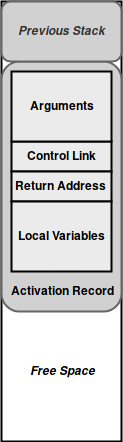
\includegraphics[scale=0.5]{figs/activation_record.png}
\caption{Activation Record 의 구조.}\label{fig:ar}
\end{figure}

먼저, 구현한 AR 의 구조는 Fig.~\ref{fig:ar} 와 같다. 각 AR 에는 순서대로 arguments, control link, return address, local variable 들이 들어간다. Local variable 이 선언될 때마다 local variable 의 길이만큼 sp 가 이동된다. 아래는 구현한 컴파일러에서 실제로 생성한 관련 코드이다.

\begin{minted}[frame=lines,
      framesep=2mm,
      baselinestretch=0.5]{asm}
  addiu $sp,$sp,-4 # allocate locals
\end{minted}

\subsection{Calling convention}

Function call 시에는 calling convention 을 따라서 runtime environement 의 적절한 처리가 필요하다. Algorithm~\ref{alg:call} 는 call sequence 를 의사코드로 표현한 것이다.

\begin{algorithm}[H]
  \caption{Call Sequence}\label{alg:call}
  \begin{enumerate}
    \item Temporary register 의 값들을 stack 에 push. \\
      $\$sp    \leftarrow sp - |\text{temporary register}_i|$ \\
      $*\$sp   \leftarrow |\text{temporary register}_i|$
    \item Argument 들을 stack 에 push. \\
      $\$sp   \leftarrow \$sp - |\text{argument}_i|$ \\
      $*\$sp \leftarrow \text{argument}_i $
    \item Caller 의 fp (callee 의 control link) 를 stack 에 push.  \\
      $\$sp \leftarrow \$sp - 4$ \\
      $*\$sp \leftarrow \$fp $
    \item Procedure 의 주소로 jump.
    \item 현재의 fp 를 sp 로 설정. \\
      $fp \leftarrow sp$
    \item Return address 를 stack에 push.\\
      $sp  \leftarrow sp - 4$ \\
      $*sp \leftarrow \$fp $
  \end{enumerate}
\end{algorithm}

아래는 구현한 컴파일러에서 실제로 출력한 어셈블리 코드의 일부이다. 위에서 묘사한 call sequence 대로 어셈블리가 생성되는 것을 볼 수 있다. Temporary register 들을 전부 stack에 push 하는건 얼핏 비효율적으로 보일 수 있다. 본 수업에서는 register allocation 을 따로 강의하지 않았고, 과제에서도 요구하지 않았기 때문에 이렇게 단순하지만 확실한 방법을 사용하였다.

\begin{minted}[frame=lines,
      framesep=2mm,
      baselinestretch=0.5]{asm}
## caller
# Save temporary registers
addiu $sp,$sp,-40
sw    $t0,0($sp)
sw    $t1,4($sp)
sw    $t2,8($sp)
sw    $t3,12($sp)
sw    $t4,16($sp)
sw    $t5,20($sp)
sw    $t6,24($sp)
sw    $t7,28($sp)
sw    $t8,32($sp)
sw    $t9,36($sp)
la    $t1, arr
addiu $sp,$sp,-4
sw    $t1,0($sp) # push argument 0
li    $t1, 45
addiu $sp,$sp,-4
sw    $t1,0($sp) # push argument 1
addiu $sp,$sp,-4
sw    $fp,0($sp) # push control link
jal   func

## callee
# set frame pointer
move  $fp,$sp
# push the return address
addiu $sp,$sp,-4
sw    $ra,0($sp)
\end{minted}

Call 이 이뤄지고, procedure 의 연산이 끝나고 나서는, 원래의 procedure 로 control 이 돌아가야 하는데, 이 작업을 return sequence 라고 한다. Algorithm~\ref{alg:ret} 는 return sequence 를 의사코드로 표현한 것이다.

\begin{algorithm}[htpb]
  \caption{Return Sequence}\label{alg:ret}
  \begin{enumerate}
    \item Return address 를 return address register 에 저장. \\
      $\$sp    \leftarrow sp - |\text{temporary register}|$ \\
      $*\$sp   \leftarrow |\text{temporary register}|$
    \item fp를 sp에 대입해서 local variable 들을 pop.  \\
      $\$sp \leftarrow \$sp - 4$ \\
      $*\$sp \leftarrow \$fp $
    \item control link 의 값을 fp 에 대입.
    \item 현재의 fp 를 sp 로 설정. \\
      $fp \leftarrow sp$
    \item Return address 의 주소로 jump.\\
      $sp  \leftarrow sp - 4$ \\
      $*sp \leftarrow \$fp $
    \item Argument 들을 stack 에서 pop. \\
      $sp \leftarrow \$fp + \sum_i |\text{argument}_i| $
    \item Temporary register 들을 stack 에서 pop. \\
      $\text{temporary register}_i \leftarrow *\$sp$ \\
      $ \$sp \leftarrow \sum_i |\text{temporary register}_i| $
    \item Return value 를 register에 저장. \\
      $ \text{register} \leftarrow \text{return value register} $

  \end{enumerate}
\end{algorithm}


아래는 구현한 컴파일러에서 실제로 출력한 어셈블리 코드의 일부이다. 위에서 묘사한 return sequence 대로 어셈블리가 생성되는 것을 볼 수 있다. Call sequence 와 대칭으로, temporary register 들의 값을 복원하는 것을 볼 수 있다.

\begin{minted}[frame=lines,
      framesep=2mm,
      baselinestretch=0.5]{asm}
## callee
# restore return address
lw    $ra,-4($fp)
# copy the fp to the sp
move  $sp,$fp
# load the control link into the fp
lw    $fp,0($fp)
# jump to the return address
j     $ra

## caller
# restore temporary registers
addiu $sp,$sp,12
lw    $t0,0($sp)
lw    $t1,4($sp)
lw    $t2,8($sp)
lw    $t3,12($sp)
lw    $t4,16($sp)
lw    $t5,20($sp)
lw    $t6,24($sp)
lw    $t7,28($sp)
lw    $t8,32($sp)
lw    $t9,36($sp)
addiu $sp,$sp,40
# load return value
move  $t1,$v0
# load return value
sw    $t1, 0($t0)
\end{minted}

\subsection{Control Statement}

\vspace{0.1in}
\noindent\textbf{if statement:} \textit{if statement} 의 경우에는 다음과 같이 코드를 생성하도록 하였다.

\begin{minted}[frame=lines,
      framesep=2mm,
      baselinestretch=0.5]{asm}
beq   $t0,$0,$_L8
# case equal ($t0 == 0)
$_L8:
# case different ($t0 != 0)
\end{minted}

\vspace{0.1in}
\noindent\textbf{if statement:} \textit{while statement} 의 경우에는 다음과 같이 코드를 생성하도록 하였다.

\begin{minted}[frame=lines,
      framesep=2mm,
      baselinestretch=0.5]{asm}
$_L10: # loop begin label
beq   $t0,$0,$_L11
# while not equal ($t0 != 0)
j     $_L10 # loop
$_L11: # loop end label
# case equal ($t0 == 0)
\end{minted}

\subsection{Register Allocation}
레지스터 할당은 다음과 같은 규칙에 따라서 할당하였다. 이를 이용해서 레지스터 할당을 수행했을 때의 syntax tree 를 Fig.~\ref{fig:reg} 에서 볼 수 있다. $r_n$ 은 할당된 레지스터의 번호이다.

\begin{align}
  child[n].r_n = parent.r_n + n
\end{align}

\begin{figure}[ht]
  \centering
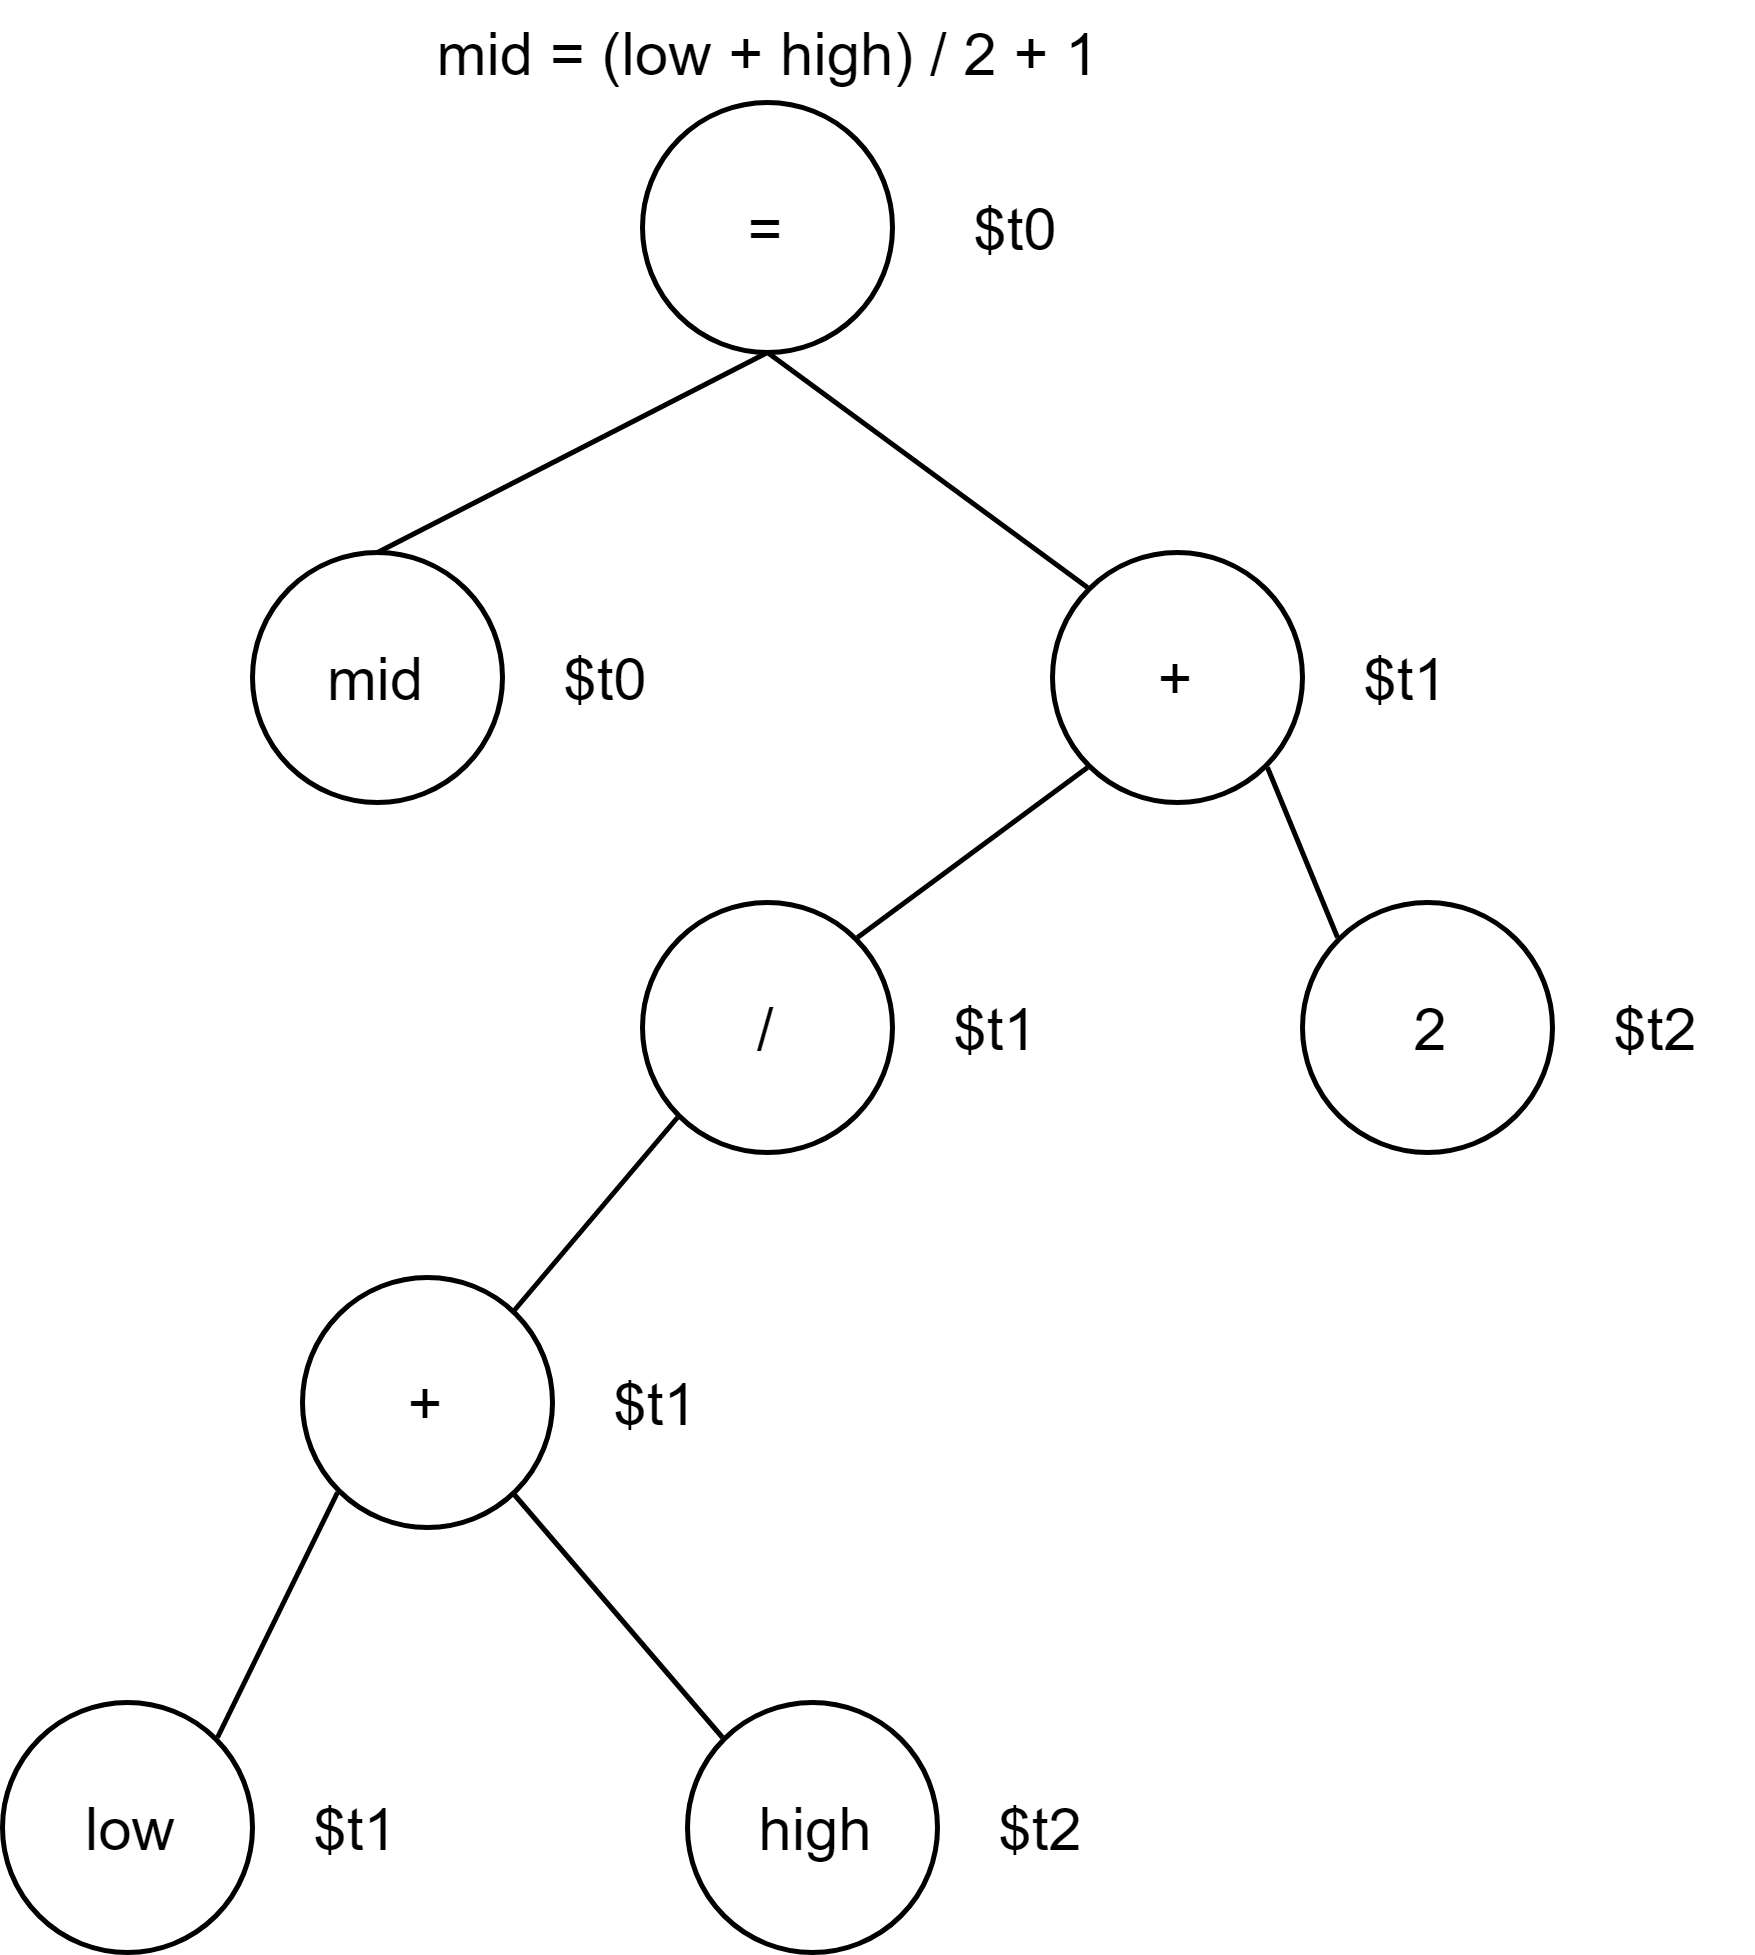
\includegraphics[scale=0.1]{figs/register.png}
\caption{Register 들을 할당한 예시.}\label{fig:reg}
\end{figure}

각 child node 의 값은 parent node 에 child 의 번호를 더한 값의 레지스터에 할당된다. 따라서 각 expression 의 dependency tree 가 오른쪽으로 degenerate 하게 형성될 경우, 레지스터 부족의 위험이 존재한다. 반대로 왼쪽으로 degenerate 하게 형성될 경우에는 레지스터 부족이 발생하지 않는다. 교수님께서 수업시간에 복잡한 프로그램은 컴파일하지 않을 것이라고 하셨기 때문에, 레지스터 부족 현상이 일어나지 않을 것이라고 가정하였다. SPIM 에서 제공하는 general purpose temporary register 는 10개 정도이기 때문에, worst-case 로 10번의 binary operation 을 수행할 경우에 레지스터 부족이 발생할 수 있다. 

\subsection{Debug Symbols}
컴파일러 커맨드라인 옵션으로 \code{--debug} 를 넣어줄 경우에는, 원본 프로그램의 소스를 해당 어셈블리 코드에 넣어주도록 하였다. 문제는 디버그 심볼을 넣는 경우에 파싱 과정에서 원본 프로그램의 소스를 읽고 또 다시 읽어서 디버그 심볼들을 추출하기 때문에 컴파일 성능이 안 좋아진다. 아래는 생성한 코드에 디버그 심볼이 들어간 모습이다.

\begin{minted}[frame=lines,
      framesep=2mm,
      baselinestretch=0.5]{asm}
#         if(parB = parA[12])
addiu $t0, $fp, 4

#         if(parB = parA[12])
li    $t2, 12
sll   $t2,$t2,2
lw    $t1, 8($fp)
addu  $t1, $t1, $t2
lw    $t1, 0($t1)
sw    $t1, 0($t0)
beq   $t0,$0,$_L2
\end{minted}

\section{분석내용}
\subsection{Test Case}\label{case}
프로그램의 정확성을 실험하기 위해 다음과 같은 테스트 파일을 만들어 테스트하였다. 다음은 첨부한 두개의 테스트 케이스중 하나인데, exponential 을 계산하는 코드이다.

\begin{minted}[frame=lines,
      framesep=2mm,
      baselinestretch=0.5]{c}
int exp(int a, int b) {
    int r;
    r = 1;
    while (b > 0) {
        r = r * a;
        b = b - 1;
    }
    return r;
}
void main(void) {
    output(exp(0-2, 10)); /* 1024  */
    output(exp(0-2, 11)); /* -2048 */
    output(exp(0-2, 12)); /* 4096 */
}
\end{minted}

위의 코드에서, \code{exp} 함수가 컴파일된 어셈블리는 아래와 같다. 컴파일이 잘 된 것을 볼 수 있다.

\begin{minted}[frame=lines,
      framesep=2mm,
      baselinestretch=0.5]{asm}
exp:
# set frame pointer
move  $fp,$sp
# push the return address
addiu $sp,$sp,-4
sw    $ra,0($sp)

addiu $sp,$sp,-4 # allocate locals


#     r = 1;
addiu $t0, $fp, -8
li    $t1, 1
sw    $t1, 0($t0)
$_L0: # loop
# evaluate the loop condition

#     while (b > 0) {
lw    $t0, 4($fp)
li    $t1, 0
slt   $t0, $t1, $t0
andi  $t0, $t0, 0x00ff
# exit if the condition is false
beq   $t0,$0,$_L1

# loop body
addiu $sp,$sp,0 # allocate locals


#         r = r * a;
addiu $t0, $fp, -8

#         r = r * a;
lw    $t1, -8($fp)
lw    $t2, 8($fp)
mult  $t1, $t2
mflo  $t1
sw    $t1, 0($t0)

#         b = b - 1;
addiu $t0, $fp, 4

#         b = b - 1;
lw    $t1, 4($fp)
li    $t2, 1
subu   $t1, $t1, $t2
sw    $t1, 0($t0)
addiu $sp,$sp,0 # free locals

j     $_L0 # loop
$_L1: # loop exit
lw    $t0, -8($fp)
move  $v0, $t0 # set return value
addiu $sp,$sp,4 # free locals


# restore return address
lw    $ra,-4($fp)
# copy the fp to the sp
move  $sp,$fp
# load the control link into the fp
lw    $fp,0($fp)
# jump to the return address
j     $ra
\end{minted}

위 예시 프로그램을 컴파일하고 실행한 모습을 Fig.~\ref{fig:screen} 에서 볼 수 있다.

\begin{figure}[ht]
  \centering
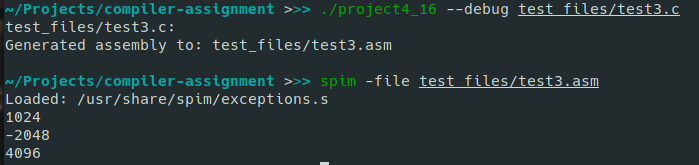
\includegraphics[scale=0.7]{figs/screenshot.png}
\caption{예시 프로그램을 컴파일하고 SPIM 으로 실행한 모습.}\label{fig:screen}
\end{figure}

이를 통해서, 컴파일이 제대로 된다는 것을 확인할 수 있따.

\section{기타}
\subsection{연구 조원 기여도}
\begin{itemize}
	\item 김규래: 50\%
	\item 박건: 50\%
\end{itemize}

\subsection{자체 평가}
디버그 심볼을 넣는 기능을 구현함으로서, 어셈블리의 코드를 편하게 디버깅할 수 있도록 하였다. 추가로 더 고급 register allocation 알고리즘을 구현했다면 더 좋았을 것 같다.

\subsection{느낀 점}
수업에서 알려주지 않은 것들이 많아서 어려움이 있었다.

\end{document}
